%=========PROBLEM 1============================================
\section*{Background}
This game revisits the classic problem of the Hunter and the Monkey. The monkey is at a distance away from the hunter. The hunter aims at the monkey at some angle and at the time he shoots, the monkey falls down from a tree. The question is at what angles will it result in a hit.

The solution to this problem can be solved analytically by utilizing the equations of motions derived from Newton's Law:
\begin{align}
    \vec{x} &= \vec{x}_0 + \Vec{v}_0*t + \frac{1}{2} \vec{a}*t^2 \\
    \vec{v} &= \vec{v}_0 + \vec{a}*t
\end{align}

Another approach is utilizing the differential form of Newton's Law, 
\begin{equation}
    \vec{F}=m\Ddot{a}
\end{equation}
and solving it numerically with the fourth order Runge-Kutta method. 

The Runge-Kutta method can be described as calculating the slope on a point an advancing a step of size $h$. Then use the previous result to calculate the slope at half step. Then, repeat but now using the last result. Then again, use the last result to calculate the slope but now advance a whole step. Finally, use the information from all the steps to calculate your next value. This process is visually explained on Figure \ref{fig:rk4Example}. Computationally, we need to program the following equation:

\begin{figure}[ht]
    \centering
    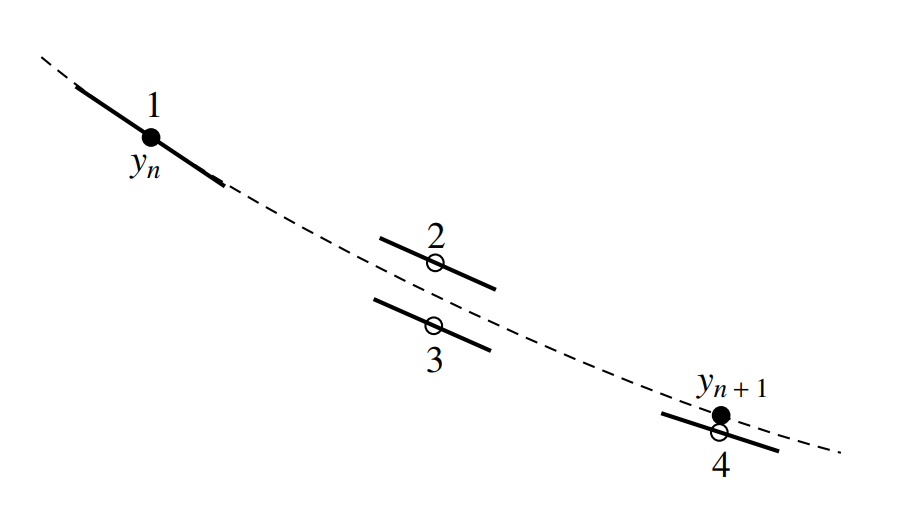
\includegraphics{rk4Example.png}
    \caption{Visually explain the fourth order Runge-Kutta method. \small{Source: Numerical Recipes 3rd Ed pg. 909}}
    \label{fig:rk4Example}
\end{figure}

\begin{align*}
    k_1 &= hf(x_n, y_n)\\
    k_2 &= hf(x_n + \frac{1}{2}h, y_n + \frac{1}{2}k_1)\\
    k_3 &= hf(x_n + \frac{1}{2}h, y_n + \frac{1}{2}k_2)\\
    k_4 &= hf(x_n + h,y_n + k_3)\\
    y_{n=1} &= y_n + \frac{1}{6}k_1 + \frac{1}{3}k_2 + \frac{1}{3}k_3 + \frac{1}{6}k_4
\end{align*}

Another approach

This differential equation can be solve by using Runge-Kutta. 


This game is comprised of 3 different play modes:

\begin{itemize}
    \item Easy: The only force acting on the bullet is the gravity.
    \item Medium: The forces acting on the bullet are gravity and air drag
    \item Difficult: The forces acting on the bullet are gravity, air resistance and a random wind.
\end{itemize}

Initial Conditions:
\begin{itemize}
    \item Horizontal distance between golfer and monkey is \SI{2000\pm 100}{\m}
    \item Vertical distance \SI{60 \pm 20}{\m}
    \item Approximate an spherical bullet with radius \SI{7.2}{\mm}
    \item Bullet mass of \SI{0.007}{\kilo\gram}
    \item Initial bullet velocity is \SI{1100}{\m\per\sec}
    \item Monkey's hit area is a circle with radius of \SI{10}{\mm}
\end{itemize}

\section*{Part 1: Easy Mode}
